% `template.tex', a bare-bones example employing the AIAA class.
%
% For a more advanced example that makes use of several third-party
% LaTeX packages, see `advanced_example.tex', but please read the
% Known Problems section of the users manual first.
%
% Typical processing for PostScript (PS) output:
%
%  latex template
%  latex template   (repeat as needed to resolve references)
%
%  xdvi template    (onscreen draft display)
%  dvips template   (postscript)
%  gv template.ps   (onscreen display)
%  lpr template.ps  (hardcopy)
%
% With the above, only Encapsulated PostScript (EPS) images can be used.
%
% Typical processing for Portable Document Format (PDF) output:
%
%  pdflatex template
%  pdflatex template      (repeat as needed to resolve references)
%
%  acroread template.pdf  (onscreen display)
%
% If you have EPS figures, you will need to use the epstopdf script
% to convert them to PDF because PDF is a limmited subset of EPS.
% pdflatex accepts a variety of other image formats such as JPG, TIF,
% PNG, and so forth -- check the documentation for your version.
%
% If you do *not* specify suffixes when using the graphicx package's
% \includegraphics command, latex and pdflatex will automatically select
% the appropriate figure format from those available.  This allows you
% to produce PS and PDF output from the same LaTeX source file.
%
% To generate a large format (e.g., 11"x17") PostScript copy for editing
% purposes, use
%
%  dvips -x 1467 -O -0.65in,0.85in -t tabloid template
%
% For further details and support, read the Users Manual, aiaa.pdf.


% Try to reduce the number of latex support calls from people who
% don't read the included documentation.
%


\typeout{}\typeout{If latex fails to find aiaa-tc, read the README file!}
%


\documentclass[]{aiaa-tc}% insert '[draft]' option to show overfull boxes
\usepackage{float}
\usepackage{epstopdf}
\usepackage{amsmath}
\usepackage[table,xcdraw]{xcolor}

\title{Attitude Estimation}

\author{
	Johnathan Clouse%
	\thanks{Graduate Student, Aerospace Engineering Sciences, 1111 Engineering Drive, Boulder, CO, 80309-0429}\\
	{\normalsize\itshape
		University of Colorado, Boulder, CO, 80309-0429, USA}
}

% Define commands to assure consistent treatment throughout document
\newcommand{\eqnref}[1]{(\ref{#1})}
\newcommand{\class}[1]{\texttt{#1}}
\newcommand{\package}[1]{\texttt{#1}}
\newcommand{\file}[1]{\texttt{#1}}
\newcommand{\BibTeX}{\textsc{Bib}\TeX}

\usepackage[euler]{textgreek}
\usepackage[colorlinks=true]{hyperref}
\hypersetup{urlcolor=cyan}

\usepackage{listings}
\usepackage{color} %red, green, blue, yellow, cyan, magenta, black, white
\definecolor{mygreen}{RGB}{28,172,0} % color values Red, Green, Blue
\definecolor{mylilas}{RGB}{170,55,241}

\usepackage{tablefootnote}
\usepackage{graphicx}
\usepackage{amsmath}
\usepackage{bm}
\usepackage{subfigure}
%\usepackage{subcaption}

\definecolor{mylilas}{RGB}{170,55,241}

% See p.105 of "TeX Unbound" for suggested values.
% See pp. 199-200 of Lamport's "LaTeX" book for details.
%   General parameters, for ALL pages:
\renewcommand{\topfraction}{0.9}	% max fraction of floats at top
\renewcommand{\bottomfraction}{0.8}	% max fraction of floats at bottom
%   Parameters for TEXT pages (not float pages):
\setcounter{topnumber}{2}
\setcounter{bottomnumber}{2}
\setcounter{totalnumber}{4}     % 2 may work better
\setcounter{dbltopnumber}{2}    % for 2-column pages
\renewcommand{\dbltopfraction}{0.9}	% fit big float above 2-col. text
\renewcommand{\textfraction}{0.07}	% allow minimal text w. figs
%   Parameters for FLOAT pages (not text pages):
\renewcommand{\floatpagefraction}{0.7}	% require fuller float pages
% N.B.: floatpagefraction MUST be less than topfraction !!
\renewcommand{\dblfloatpagefraction}{0.7}	% require
    \makeatletter
    \renewcommand\l@section{\@dottedtocline{2}{1.5em}{3em}}
    \makeatother
    
\begin{document}
	

	
	\maketitle
	
	\begin{abstract}
		\noindent 
		
	\end{abstract}
	
	\newpage
	
	\tableofcontents
	
	\newpage

	\section{Introduction}
Jupiter is the largest planet in the solar system, and the closest gas giant to the sun. It is a planet that is rich with opportunities for scientific inquiry. Jupiter's makeup can give clues to how the solar system was created. The largest moon, Ganymede, is thought to have a subsurface ocean and an active core. Europa also has a subsurface ocean, and geysers that spout water far above the surface. Either of these moons could hold life, but the first step in exploring them is to reach the Jupiter system.
	
	\section{Attitude Dynamics}
	\begin{equation}
		\begin{matrix}
		I_{11}\dot{\omega_1}=-(I_{33}-I_{22})\omega_2\omega_3+T_1\\ 
		I_{22}\dot{\omega_2}=-(I_{11}-I_{33})\omega_3\omega_1+T_2\\ 
		I_{33}\dot{\omega_3}=-(I_{22}-I_{11})\omega_1\omega_2+T_3
		\end{matrix}
		\label{eqn:EOM}
	\end{equation}

	\begin{equation}		
		\begin{pmatrix}
		\dot{\psi}\\ 
		\dot{\theta}\\ 
		\dot{\phi}
		\end{pmatrix} = 
		\frac{1}{\cos \theta}\begin{bmatrix}
		0 & \sin\phi & \cos\phi \\ 
		0 & \cos\phi\cos\theta & -\sin\phi\cos\theta\\ 
		\cos \theta & \sin\phi\sin\theta & \cos\phi\sin\theta
		\end{bmatrix}
		\begin{pmatrix}
		\omega_1\\ 
		\omega_2\\ 
		\omega_3
		\end{pmatrix}=
		B(\psi,\theta\phi)\boldsymbol{\omega}
		\label{eqn:diffEqEuler}
	\end{equation}

	\begin{equation}
		DCM_{YPR} = \begin{bmatrix}
		\cos\theta\cos\psi & \cos\theta\sin\psi & -\sin\theta\\ 
		\sin\phi\sin\theta\cos\psi -\cos\phi\sin\psi& \sin\phi\sin\theta\sin\psi+\cos\phi\cos\psi & \sin\phi\cos\theta\\ 
		\cos\phi\sin\theta\cos\psi+\sin\phi\sin\psi & \cos\phi\sin\theta\sin\psi-\sin\phi\cos\psi & cos\phi\cos\theta
		\end{bmatrix}
		\label{eqn:DCM_Euler}
	\end{equation}

	\begin{equation}
		\vec{T}_{grav} = \frac{3\mu}{R^5}\begin{pmatrix}
		R_2R_3(I_{33}-I_{22})\\ 
		R_1R_3(I_{11}-I_{33})\\ 
		R_1R_2(I_{22}-I_{11})
		\end{pmatrix}
		\label{eqn:GGTorque}
	\end{equation}

	\begin{equation}
		\begin{pmatrix}
		\dot{\psi}\\ 
		\dot{\theta}\\ 
		\dot{\phi}
		\end{pmatrix} = 
		B(\psi,\theta\phi)\boldsymbol{\omega}-\frac{\Omega}{\cos\theta}\begin{pmatrix}
		\sin\theta\sin\psi\\ 
		-\cos\theta\cos\psi\\ 
		-\sin\psi
		\end{pmatrix}
		\label{eqn:EulerGGDiffEq}
	\end{equation}
	\section{Simulation}

A microsatellite in low Earth orbit was simulated to provide data to be filtered. The simulated state was comprised of Earth-inertial position and velocity, the inertial-to-body quaternion, and the inertial rates expressed in the body frame. Position and velocity were propagated with a two-body point-mass model, while attitude was propagated with gravity gradient torque using Equations \ref{eqn:EOM} and \ref{eqn:GGTorque}. Table \ref{table:SimParams} lists the parameter values that were used in the simulation.

% Please add the following required packages to your document preamble:
% \usepackage[table,xcdraw]{xcolor}
% If you use beamer only pass "xcolor=table" option, i.e. \documentclass[xcolor=table]{beamer}
\begin{table}[H]
\centering
\caption{Simulation Parameters}
\label{table:SimParams}
\begin{tabular}{|l|l|}
\rowcolor[HTML]{C0C0C0} 
\textbf{Parameter}                                                                    & \textbf{Value} \\ \hline
Orbit Semi-major axis                                                                 & 6678 km        \\ \hline
Orbit Eccentricity                                                                    & 0              \\ \hline
Orbit Inclination                                                                     & 23$^\circ$             \\ \hline
Orbit Arg of Periapse                                                                 & 0$^\circ$              \\ \hline
\begin{tabular}[c]{@{}l@{}}Orbit Right Ascention\\ of the Ascending Node\end{tabular} & 0$^\circ$              \\ \hline
Initial true anomaly                                                                  & 0$^\circ$              \\ \hline
Spacecraft Mass                                                                       & 50 kg          \\ \hline
Spacecraft Length                                                                     & 0.5 m          \\ \hline
Spacecraft Width                                                                      & 0.316 m             \\ \hline
$\mu_{Earth}$                                                                      & 3.986e5 km            \\ \hline
\end{tabular}
\end{table}

The results of the simulation are shown in Figure \ref{fig:SimResults} below.
	\begin{figure}[H]
		\centering
		\subfigure[Euler angles wrt LVLH]{
			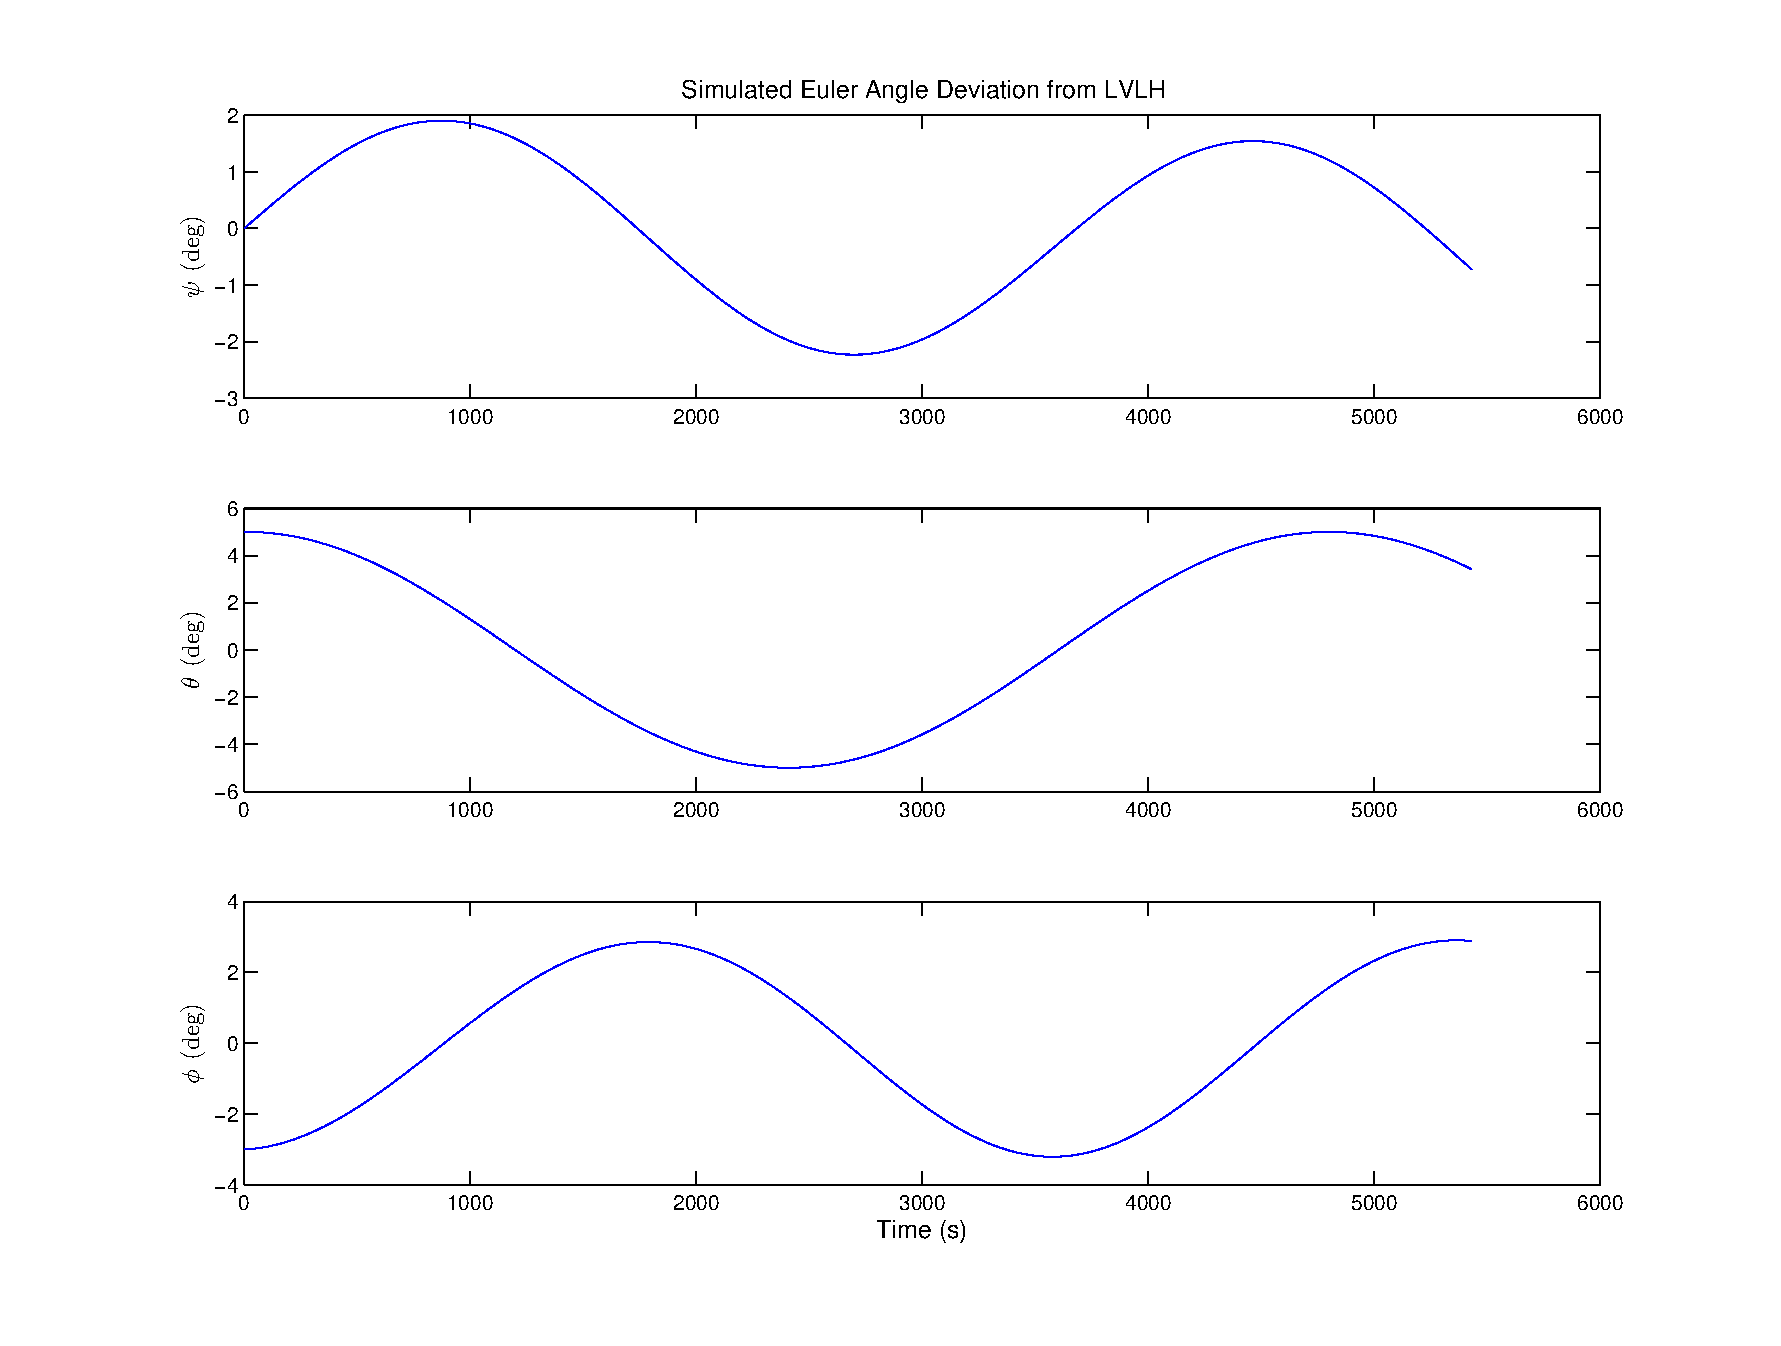
\includegraphics[width = 12cm]{../Figures/sim_angles.eps}
		}
		\subfigure[Body Rates]{
			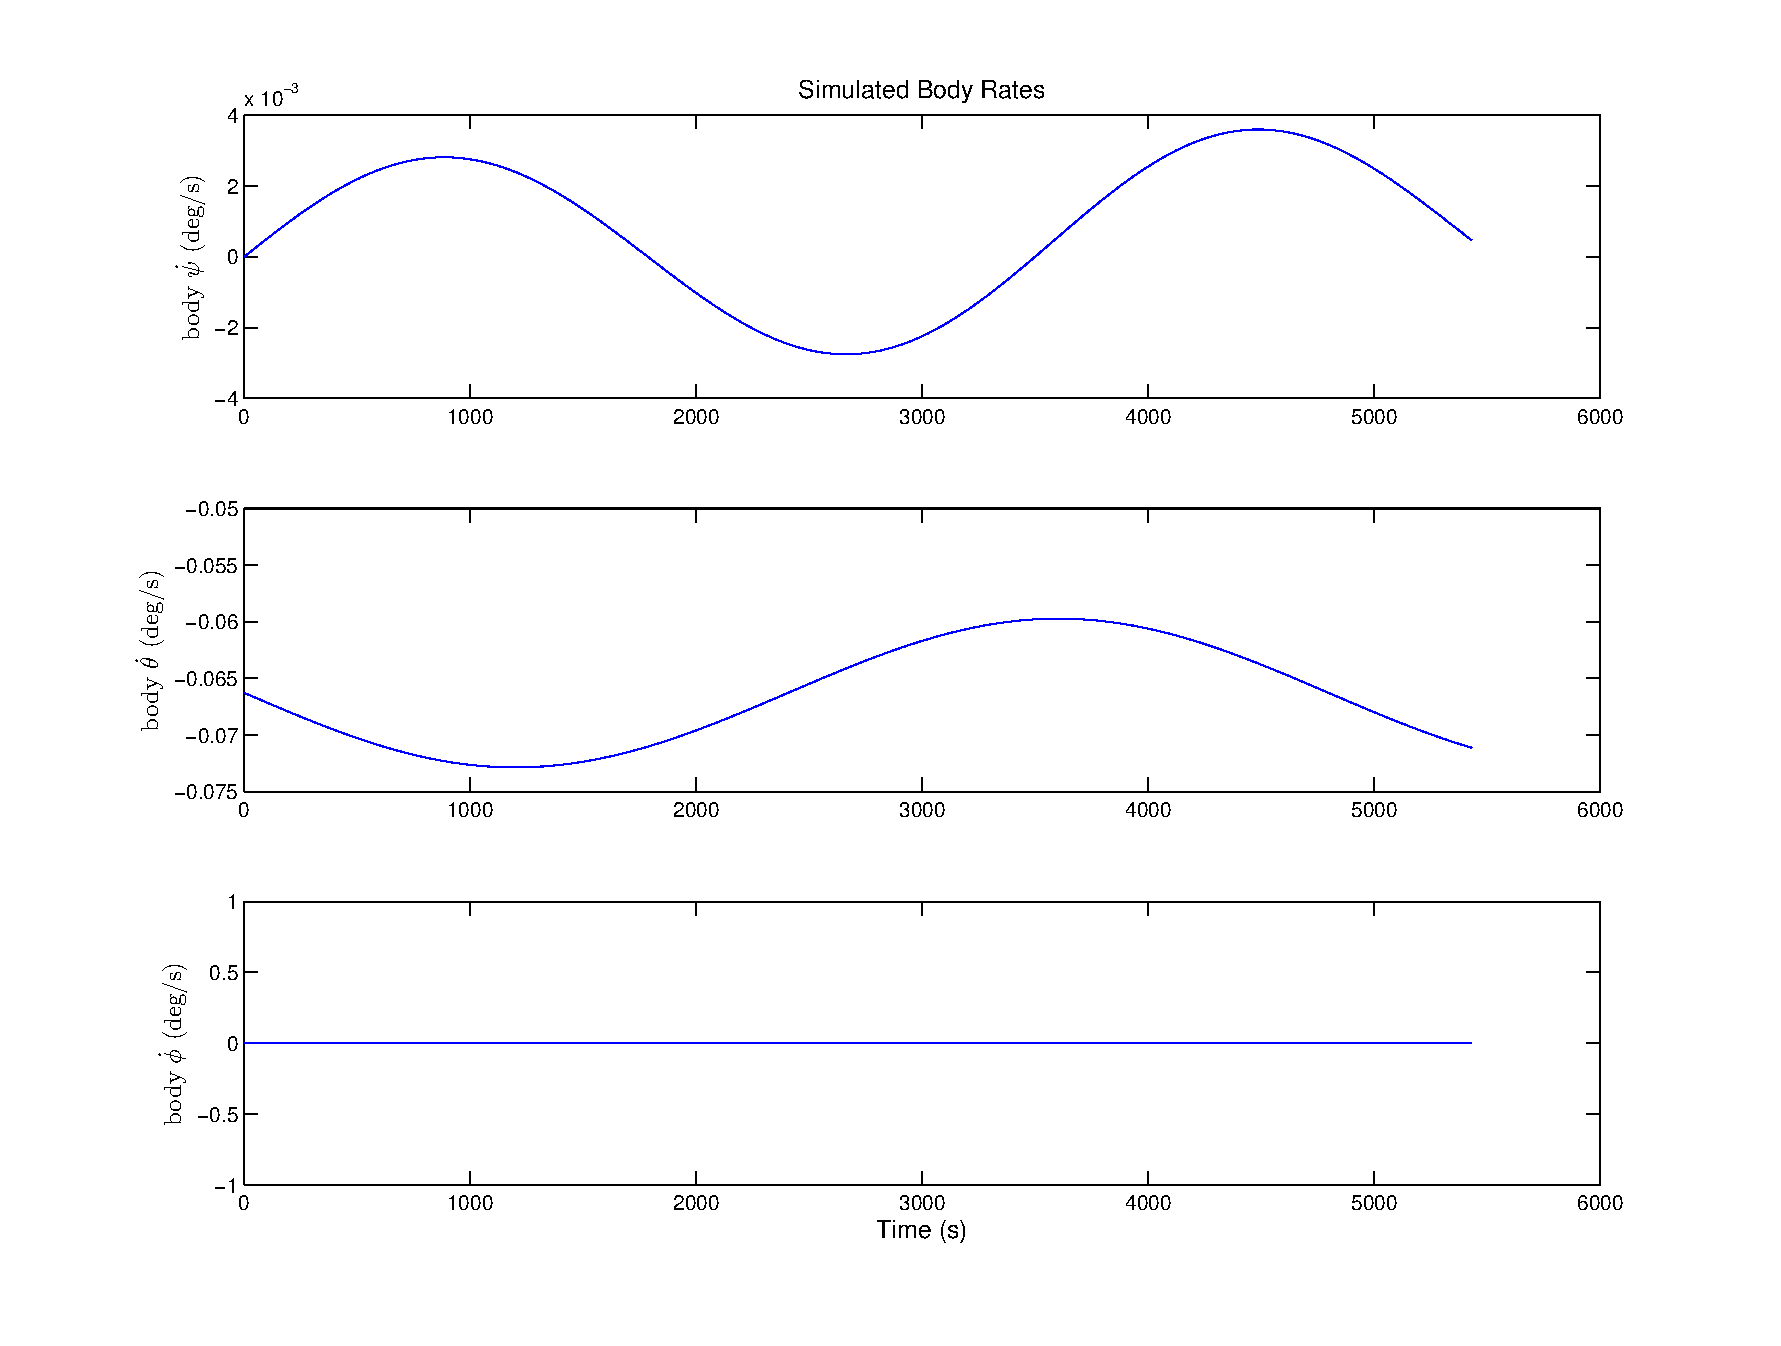
\includegraphics[width = 12cm]{../Figures/sim_rates.eps}
		}
		\caption{Simulation results }
		\label{fig:SimResults}
	\end{figure}	

As expected, the gravity-gradient torque produced an oscillatory motion about the pitch and roll axes. The body yaw rate stays at zero due to the spacecraft symmetry, but the yaw in the euler representation is non-zero because it's a component of the attitude representation.

	\section{Filtering the Euler Representation}

	\section{Conclusion}

	A trajectory to Jupiter was found that met all requirements was found. An algorithm was developed to find the trajectory, but improvements could still be made. Implementing a genetic algorithm or a minimization routine could reduce processing time for the algorithm. Further, the algorithm was implemented as a single thread; a multi-threaded version of the algorithm could also reduce search time.

	\vspace{5 mm}

The trajectory was proven to work in STK. However, the TCMs became large in the end. This is due to the difference in ephemerides the algorithm and STK used, as well as STK's higher-fidelity modeling. Future would should implement JPL's SPICE kernel to make use of similar ephemerides to STK. Additionally, running the algorithm with a smaller window granularity could lower the STK-calculated TCMs. Incorporating these calculations into STK through its custom interfaces could make it easier to target a gravity assist with smaller TCMs required.

	\vspace{5 mm}

Earth access for this trajectory was computed for various events in the mission. During cruise, there is always DSN access when the sun is not in conjunction. The Venus gravity assist was visible to the Goldstone and Madrid facilities. For the Earth gravity assists, there was access except for a short time around the closest approach. However, even though there was line of sight between the spacecraft and the ground stations, the dynamics of the spacecraft flying quickly past the Earth could make it difficult for the DSN antennae to truly maintain access.  Due to the favorable geometry of the final transfer to Jupiter, JOI could be targeted to give access to any two DSN facilities. 

	\vspace{5 mm}

Maneuvers to explore the Jupiter system were studied. First, a direct transfer from the initial Jovian orbit to Europa capture was considered. With a required $\Delta$V on the scale produced by launch vehicles, this was not feasible. Next, Ganymede was used to lower apojove. Although the first maneuver performed to fly by Ganymede had a large out-of-plane component, it was shown that using this moon to reduce orbit energy was much more efficient than impulsive $\Delta$Vs at perijove. A targeting algorithm with realistic ephemerides could lower the TCM $\Delta$V even further.

	\vspace{5 mm}

Mission design is a complex process that is part art, and part science. Trial and error were invoked many times through the course of this investigation, as the dynamics and timescales involved are beyond the implementation of a simple algorithm. With a firm grasp of the underlying mechanics, one can effectively utilize hardware computation after removing unrealistic scenarios from consideration. The subsequent fine-tuning will allow for a cost-efficient mission that can meet and exceed its stated goals.


\bibliographystyle{aiaa}   % Number the references.
\bibliography{ASEN6080ProjectBib}   % Use references.bib to resolve the labels.

%    \section{Appendix B}
%This appendix contains all Matlab code used by the authors to analyize their data.
%    
%    \lstset{language=Matlab,%
%    	%basicstyle=\color{red},
%    	breaklines=true,%
%    	morekeywords={matlab2tikz},
%    	keywordstyle=\color{blue},%
%    	morekeywords=[2]{1}, keywordstyle=[2]{\color{black}},
%    	identifierstyle=\color{black},%
%    	stringstyle=\color{mylilas},
%    	commentstyle=\color{mygreen},%
%    	showstringspaces=false,%without this there will be a symbol in the places where there is a space
%    	numbers=left,%
%    	numberstyle={\tiny \color{black}},% size of the numbers
%    	numbersep=9pt, % this defines how far the numbers are from the text
%    	emph=[1]{for,end,break},emphstyle=[1]\color{red}, %some words to emphasise
%    	%emph=[2]{word1,word2}, emphstyle=[2]{style},   
%    }
    
%    \lstinputlisting{ASEN5090_ecef2azelrange.m}
%    \vspace{5mm}
%    
%    \lstinputlisting{ASEN5090_GPSvis.m}
%    \vspace{5mm}
%\lstinputlisting{HW5_rel_err.m}
%\vspace{5mm}
%\lstinputlisting{import_gps_data.m}
%\vspace{5mm}
%\lstinputlisting{datenum8601.m}
%\vspace{5mm}
%\lstinputlisting{lab_err_plots.m}
%\vspace{5mm}
	
\end{document}

% - Release $Name:  $ -
